\def\slidemode{%
  \documentclass[fleqn,aspectratio=169]{beamer}
}
\def\handoutmode{%
  \documentclass[handout,fleqn,aspectratio=169]{beamer}
}

\def\slidemode{
  \documentclass[fleqn,aspectratio=169]{beamer}
\usepackage{pgfpages}
}
\def\handoutmode{
  \documentclass[handout,fleqn,aspectratio=169]{beamer}
\usepackage{pgfpages}
\pgfpagesuselayout{resize to}[a4paper,landscape,border shrink=5mm]
}


%\def\pdfmode{handoutmode}
\def\pdfmode{slidemode}

\csname\pdfmode\endcsname

% when making printed slides
\usepackage{pgfpages}
\pgfpagesuselayout{resize to}[a4paper,landscape,border shrink=5mm]


\mode<presentation>
{
  \usetheme{default}
  \usecolortheme{default}
  \usefonttheme{default}
  \setbeamertemplate{navigation symbols}{}
  \setbeamertemplate{caption}[numbered]
  \setbeamertemplate{footline}[frame number]  % or "page number"
  \setbeamercolor{frametitle}{fg=white}
  \setbeamercolor{footline}{fg=black}
} 

\usepackage[english]{babel}
%\usepackage[utf8x]{inputenc}
\usepackage{tikz}
\usepackage{courier}
\usepackage{array}
\usepackage{bold-extra}
%\usepackage{minted}
%\usepackage[thicklines]{cancel}
%\usepackage{fancyvrb}
\usepackage{kotex}
\usepackage{paralist}
\usepackage{collectbox}
\usepackage{amsmath}
\usepackage{mathtools}

\setbeamercolor{block body alerted}{bg=alerted text.fg!10}
\setbeamercolor{block title alerted}{bg=alerted text.fg!20}
\setbeamercolor{block body}{bg=structure!10}
\setbeamercolor{block title}{bg=structure!20}
\setbeamercolor{block body example}{bg=green!10}
\setbeamercolor{block title example}{bg=green!20}
\setbeamertemplate{blocks}[rounded][shadow]

\xdefinecolor{dianablue}{rgb}{0.18,0.24,0.31}
\xdefinecolor{darkblue}{rgb}{0.1,0.1,0.7}
\xdefinecolor{darkgreen}{rgb}{0,0.5,0}
\xdefinecolor{darkgrey}{rgb}{0.35,0.35,0.35}
\xdefinecolor{darkorange}{rgb}{0.8,0.5,0}
\xdefinecolor{darkred}{rgb}{0.7,0,0}
\definecolor{darkgreen}{rgb}{0,0.6,0}
\definecolor{mauve}{rgb}{0.58,0,0.82}


\makeatletter
\setbeamertemplate{footline}
{
  \leavevmode%
  \hbox{%
  \begin{beamercolorbox}[wd=.333333\paperwidth,ht=2.25ex,dp=1ex,center]{author in head/foot}%
    \usebeamerfont{author in head/foot}\insertsection
  \end{beamercolorbox}%
  \begin{beamercolorbox}[wd=.333333\paperwidth,ht=2.25ex,dp=1ex,center]{title in head/foot}%
    \usebeamerfont{title in head/foot}\insertsubsection
  \end{beamercolorbox}%
  \begin{beamercolorbox}[wd=.333333\paperwidth,ht=2.25ex,dp=1ex,right]{date in head/foot}%
    \usebeamerfont{date in head/foot}
    \insertshortdate{}\hspace*{2em}
    \insertframenumber{} / \inserttotalframenumber\hspace*{2ex} 
  \end{beamercolorbox}}%

  \vskip0pt%
}
\makeatother

\title[]{Lecture 1: Probabilistic Model}
\author{Yi, Yung (이융)}
\institute{EE210: Probability and Introductory Random Processes\\ KAIST EE}
\date{\today}

\usetikzlibrary{shapes.callouts}

%%%%%%%%%%%% real, integer notation
\newcommand{\real}{{\mathbb R}}
\newcommand{\integer}{{\mathbb Z}}

%%% set, vector, matrix
\newcommand{\set}[1]{\ensuremath{\mathcal #1}}
\renewcommand{\vec}[1]{\bm{#1}}
\newcommand{\mat}[1]{\bm{#1}}


%%% big parenthesis
\def\Bl{\Bigl}
\def\Br{\Bigr}
\def\lf{\left}
\def\ri{\right}


%%% floor notations
\newcommand{\lfl}{{\lfloor}}
\newcommand{\rfl}{{\rfloor}}
\newcommand{\floor}[1]{{\lfloor #1 \rfloor}}

%%% gradient
\newcommand{\grad}[1]{\nabla #1}

%%% definition
\newcommand{\eqdef}{\ensuremath{\triangleq}}
%%% imply
\newcommand{\imp}{\Longrightarrow}



\newcommand{\separator}{
%  \begin{center}
    \par\noindent\rule{\columnwidth}{0.3mm}
%  \end{center}
}

\newcommand{\mynote}[1]{{\it \color{red} [#1]}}







%%% equation alignment
\newcommand{\aleq}[1]{\begin{align*}#1\end{align*}}

%%%%%%%%%%%%%%%% colored emphasized font, blanked words

\newcommand{\empr}[1]{{\color{red}\emph{#1}}}
\newcommand{\empb}[1]{{\color{blue}\emph{#1}}}

%normal colored text
\newcommand{\redf}[1]{{\color{red} #1}}
\newcommand{\yellowf}[1]{{\color{yellow} #1}}
\newcommand{\bluef}[1]{{\color{blue} #1}}
\newcommand{\grayf}[1]{{\color{gray} #1}}
\newcommand{\magenf}[1]{{\color{magenta} #1}}
\newcommand{\greenf}[1]{{\color{green} #1}}
\newcommand{\cyanf}[1]{{\color{cyan} #1}}
\newcommand{\orangef}[1]{{\color{orange} #1}}


\newcommand{\blk}[1]{\underline{\mbox{\hspace{#1}}}}


\newcommand{\redblk}[1]{\framebox{\color{red} #1}}
\newcommand{\redblank}[2]{\framebox{\onslide<#1->{\color{red} #2}}}
\newcommand{\blueblk}[1]{\framebox{\color{blue} #1}}
\newcommand{\blueblank}[2]{\framebox{\onslide<#1->{\color{blue} #2}}}



\makeatletter
\newcommand{\mybox}{%
    \collectbox{%
        \setlength{\fboxsep}{1pt}%
        \fbox{\BOXCONTENT}%
    }%
}
\makeatother

\makeatletter
\newcommand{\lecturemark}{%
    \collectbox{%
        \setlength{\fboxsep}{1pt}%
        \fcolorbox{red}{yellow}{\BOXCONTENT}%
    }%
}
\makeatother

\usepackage{tcolorbox}
\newcommand{\mycolorbox}[1]{
\begin{tcolorbox}[colback=red!5!white,colframe=red!75!black]
#1
\end{tcolorbox}
}

%%%% figure inclusion
\newcommand{\mypic}[2]{
\begin{center}
\includegraphics[width=#1\textwidth]{#2}
\end{center}
}

\newcommand{\myinlinepic}[2]{
\makebox[0cm][r]{\raisebox{-4ex}{\includegraphics[height=#1]{#2}}}
}


%%%% itemized and enumerated list
\newcommand{\bci}{\begin{compactitem}}
\newcommand{\eci}{\end{compactitem}}
\newcommand{\bce}{\begin{compactenum}}
\newcommand{\ece}{\end{compactenum}}


%%%% making 0.5/0.5 two columns
%%%% how to use: first number: length of separation bar
% \mytwocols{0.6}
% {
% contents in the left column
% }
% {
% contents in the right column
% }
%%%%
\newcommand{\mytwocols}[3]{
\begin{columns}[T] \column{.499\textwidth} #2 \column{.001\textwidth} \rule{.3mm}{{#1}\textheight} \column{.499\textwidth} #3 \end{columns}}

\newcommand{\mythreecols}[4]{
\begin{columns}[T] \column{.31\textwidth} #2 \column{.001\textwidth} \rule{.3mm}{{#1}\textheight} \column{.31\textwidth} #3 \column{.001\textwidth} \rule{.3mm}{{#1}\textheight} \column{.31\textwidth} #4  \end{columns}}

\newcommand{\mysmalltwocols}[3]{
\begin{columns}[T] \column{.4\textwidth} #2 \column{.001\textwidth} \rule{.3mm}{{#1}\textheight} \column{.4\textwidth} #3 \end{columns}}

%%%% making two columns with customized ratios
%%%% how to use:
%first parameter: length of separation bar
%second parameter: ratio of left column
%third parameter: ratio of right column
% \mytwocols{0.6}{0.7}{0.29}
% {
% contents in the left column
% }
% {
% contents in the right column
% }
%%%%
\newcommand{\myvartwocols}[5]{
\begin{columns}[T] \column{#2\textwidth} {#4} \column{.01\textwidth} \rule{.3mm}{{#1}\textheight} \column{#3\textwidth} {#5} \end{columns}}

%%% making my block in beamer
%%% first parameter: title of block
%%% second parameter: contents of block
\newcommand{\myblock}[2]{
\begin{block}{#1} {#2}  \end{block}}

%%% independence notation
\newcommand{\indep}{\perp \!\!\! \perp}

%%%% probability with different shapes (parenthesis or bracket) and different sizes
%%% `i' enables us to insert the subscript to the probability
\newcommand{\bprob}[1]{\mathbb{P}\Bl[ #1 \Br]}
\newcommand{\prob}[1]{\mathbb{P}[ #1 ]}
\newcommand{\cbprob}[1]{\mathbb{P}\Bl( #1 \Br)}
\newcommand{\cprob}[1]{\mathbb{P}( #1 )}
\newcommand{\probi}[2]{\mathbb{P}_{#1}[ #2 ]}
\newcommand{\bprobi}[2]{\mathbb{P}_{#1}\Bl[ #2 \Br]}
\newcommand{\cprobi}[2]{\mathbb{P}_{#1}( #2 )}
\newcommand{\cbprobi}[2]{\mathbb{P}_{#1}\Bl( #2 \Br)}

%%%% expectation with different shapes (parenthesis or bracket) and different sizes
%%% `i' enables us to insert the subscript to the expectation
\newcommand{\expect}[1]{\mathbb{E}[ #1 ]}
\newcommand{\cexpect}[1]{\mathbb{E}( #1 )}
\newcommand{\bexpect}[1]{\mathbb{E}\Bl[ #1 \Br]}
\newcommand{\cbexpect}[1]{\mathbb{E}\Bl( #1 \Br)}
\newcommand{\bbexpect}[1]{\mathbb{E}\lf[ #1 \ri]}
\newcommand{\expecti}[2]{\mathbb{E}_{#1}[ #2 ]}
\newcommand{\bexpecti}[2]{\mathbb{E}_{#1}\Bl[ #2 \Br]}
\newcommand{\bbexpecti}[2]{\mathbb{E}_{#1}\lf[ #2 \ri]}

%%%% variance
\newcommand{\var}[1]{\text{var}[ #1 ]}
\newcommand{\bvar}[1]{\text{var}\Bl[ #1 \Br]}
\newcommand{\cvar}[1]{\text{var}( #1 )}
\newcommand{\cbvar}[1]{\text{var}\Bl( #1 \Br)}

%%%% covariance
\newcommand{\cov}[1]{\text{cov}( #1 )}
\newcommand{\bcov}[1]{\text{cov}\Bl( #1 \Br)}

%%% Popular pmf, pdf notation to avoid long typing
\newcommand{\px}{\ensuremath{p_X(x)}}
\newcommand{\py}{\ensuremath{p_Y(y)}}
\newcommand{\pz}{\ensuremath{p_Z(z)}}
\newcommand{\pxA}{\ensuremath{p_{X|A}(x)}}
\newcommand{\pyA}{\ensuremath{p_{Y|A}(y)}}
\newcommand{\pzA}{\ensuremath{p_{Z|A}(z)}}
\newcommand{\pxy}{\ensuremath{p_{X,Y}(x,y)}}
\newcommand{\pxcy}{\ensuremath{p_{X|Y}(x|y)}}
\newcommand{\pycx}{\ensuremath{p_{Y|X}(y|x)}}

\newcommand{\fx}{\ensuremath{f_X(x)}}
\newcommand{\Fx}{\ensuremath{F_X(x)}}
\newcommand{\fy}{\ensuremath{f_Y(y)}}
\newcommand{\Fy}{\ensuremath{F_Y(y)}}
\newcommand{\fz}{\ensuremath{f_Z(z)}}
\newcommand{\Fz}{\ensuremath{F_Z(z)}}
\newcommand{\fxA}{\ensuremath{f_{X|A}(x)}}
\newcommand{\fyA}{\ensuremath{f_{Y|A}(y)}}
\newcommand{\fzA}{\ensuremath{f_{Z|A}(z)}}
\newcommand{\fxy}{\ensuremath{f_{X,Y}(x,y)}}
\newcommand{\Fxy}{\ensuremath{F_{X,Y}(x,y)}}
\newcommand{\fxcy}{\ensuremath{f_{X|Y}(x|y)}}
\newcommand{\fycx}{\ensuremath{f_{Y|X}(y|x)}}

\newcommand{\fth}{\ensuremath{f_\Theta(\theta)}}
\newcommand{\fxcth}{\ensuremath{f_{X|\Theta}(x|\theta)}}
\newcommand{\fthcx}{\ensuremath{f_{\Theta|X}(\theta|x)}}

\newcommand{\pkcth}{\ensuremath{p_{X|\Theta}(k|\theta)}}
\newcommand{\fthck}{\ensuremath{f_{\Theta|X}(\theta|k)}}


%%%% indicator
\newcommand{\indi}[1]{\mathbf{1}_{ #1 }}

%%%% exponential rv.
\newcommand{\elambdax}{\ensuremath{e^{-\lambda x}}}

%%%% normal  rv.
\newcommand{\stdnormal}{\ensuremath{\frac{1}{\sqrt{2\pi}} e^{-x^2/2}}}
\newcommand{\gennormal}{\ensuremath{\frac{1}{\sigma\sqrt{2\pi}} e^{-(x-\mu)^2/2}}}

%%%%%% estimator, estimate
\newcommand{\hth}{\ensuremath{\hat{\theta}}}
\newcommand{\hTH}{\ensuremath{\hat{\Theta}}}
\newcommand{\MAP}{\ensuremath{\text{MAP}}}
\newcommand{\LMS}{\ensuremath{\text{LMS}}}
\newcommand{\LLMS}{\ensuremath{\text{L}}}
\newcommand{\ML}{\ensuremath{\text{ML}}}

%%%% colored text
\newcommand{\red}[1]{\color{red}#1}
\newcommand{\cyan}[1]{\color{cyan}#1}
\newcommand{\magenta}[1]{\color{magenta}#1}
\newcommand{\blue}[1]{\color{blue}#1}
\newcommand{\green}[1]{\color{green}#1}
\newcommand{\white}[1]{\color{white}#1}

\newcommand{\defi}{{\color{red} Definition.} }
\newcommand{\proff}{{\color{red} Proof.} }
\newcommand{\exam}{{\color{red} Example.} }
\newcommand{\question}{{\color{red} Question.} }
\newcommand{\thm}{{\color{red} Theorem.} }
\newcommand{\background}{{\color{red} Background.} }
\newcommand{\msg}{{\color{red} Message.} }

\newcommand{\bern}[1]{\ensuremath{\text{Bern}(#1)} }
\newcommand{\bp}[1]{\ensuremath{\text{BP}(#1)} }
\newcommand{\poisson}[1]{\ensuremath{\text{Poisson}(#1)} }
\newcommand{\pp}[1]{\ensuremath{\text{PP}(#1)} }


%%%%%%%%%%%%%%%%%%%%%%% old macros that you can ignore %%%%%%%%%%%%%%%%%%%%%%%%

% \def\un{\underline}
% \def\ov{\overline}


% \newcommand{\beq}{\begin{eqnarray*}}
% \newcommand{\eeq}{\end{eqnarray*}}
% \newcommand{\beqn}{\begin{eqnarray}}
% \newcommand{\eeqn}{\end{eqnarray}}
% \newcommand{\bemn}{\begin{multiline}}
% \newcommand{\eemn}{\end{multiline}}
% \newcommand{\beal}{\begin{align}}
% \newcommand{\eeal}{\end{align}}
% \newcommand{\beas}{\begin{align*}}
% \newcommand{\eeas}{\end{align*}}



% \newcommand{\bd}{\begin{displaymath}}
% \newcommand{\ed}{\end{displaymath}}
% \newcommand{\bee}{\begin{equation}}
% \newcommand{\eee}{\end{equation}}


% \newcommand{\vs}{\vspace{0.2in}}
% \newcommand{\hs}{\hspace{0.5in}}
% \newcommand{\el}{\end{flushleft}}
% \newcommand{\bl}{\begin{flushleft}}
% \newcommand{\bc}{\begin{center}}
% \newcommand{\ec}{\end{center}}
% \newcommand{\remove}[1]{}

% \newtheorem{theorem}{Theorem}
% \newtheorem{corollary}{Corollary}
% \newtheorem{prop}{Proposition}
% \newtheorem{lemma}{Lemma}
% \newtheorem{defi}{Definition}
% \newtheorem{assum}{Assumption}
% \newtheorem{example}{Example}
% \newtheorem{property}{Property}
% \newtheorem{remark}{Remark}

% \newcommand{\separator}{
%   \begin{center}
%     \rule{\columnwidth}{0.3mm}
%   \end{center}
% }

% \newenvironment{separation}
% { \vspace{-0.3cm}
%   \separator
%   \vspace{-0.25cm}
% }
% {
%   \vspace{-0.5cm}
%   \separator
%   \vspace{-0.15cm}
% }

% \def\A{\mathcal A}
% \def\oA{\overline{\mathcal A}}
% \def\S{\mathcal S}
% \def\D{\mathcal D}
% \def\eff{{\rm Eff}}
% \def\bD{\bm{D}}
% \def\cU{{\cal U}}
% \def\bbs{{\mathbb{s}}}
% \def\bbS{{\mathbb{S} }}
% \def\cM{{\cal M}}
% \def\bV{{\bm{V}}}
% \def\cH{{\cal H}}
% \def\ch{{\cal h}}
% \def\cR{{\cal R}}
% \def\cV{{\cal V}}
% \def\cA{{\cal A}}
% \def\cX{{\cal X}}
% \def\cN{{\cal N}}
% \def\cJ{{\cal J}}
% \def\cK{{\cal K}}
% \def\cL{{\cal L}}
% \def\cI{{\cal I}}
% \def\cY{{\cal Y}}
% \def\cZ{{\cal Z}}
% \def\cC{{\cal C}}
% \def\cR{{\cal R}}
% \def\id{{\rm Id}}
% \def\st{{\rm st}}
% \def\cF{{\cal F}}
% \def\bz{{\bm z}}
% \def\cG{{\cal G}}
% \def\N{\mathbb{N}}
% \def\bbh{\mathbb{h}}
% \def\bbH{\mathbb{H}}
% \def\bbi{\mathbb{i}}
% \def\bbI{\mathbb{I}}
% \def\R{\mathbb{R}}
% \def\bbR{\mathbb{R}}
% \def\bbr{\mathbb{r}}
% \def\cB{{\cal B}}
% \def\cP{{\cal P}}
% \def\cS{{\cal S}}
% \def\bW{{\bm W}}
% \def\bc{{\bm c}}

% %\def\and{\quad\mbox{and}\quad}
% \def\ind{{\bf 1}}


% \def\bmg{{\bm{\gamma}}}
% \def\bmr{{\bm{\rho}}}
% \def\bmq{{\bm{q}}}
% \def\bmt{{\bm{\tau}}}
% \def\bmn{{\bm{n}}}
% \def\bmcapn{{\bm{N}}}
% \def\bmrho{{\bm{\rho}}}

% \def\igam{\underline{\gamma}(\lambda)}
% \def\sgam{\overline{\gamma}(\lambda)}
% \def\ovt{\overline{\theta}}
% \def\ovT{\overline{\Theta}}
% \def\PP{{\mathrm P}}
% \def\EE{{\mathrm E}}
% \def\iskip{{\vskip -0.4cm}}
% \def\siskip{{\vskip -0.2cm}}

% \def\bp{\noindent{\it Proof.}\ }
% \def\ep{\hfill $\Box$}



%\renewcommand{\baselinestretch}{2.0}

\begin{document}

%itemshape
\setbeamertemplate{itemize item}{\scriptsize\raise1.25pt\hbox{\donotcoloroutermaths$\bullet$}}
\setbeamertemplate{itemize subitem}{\tiny\raise1.5pt\hbox{\donotcoloroutermaths$\circ$}}
\setbeamertemplate{itemize subsubitem}{\tiny\raise1.5pt\hbox{\donotcoloroutermaths$\blacktriangleright$}}
%default value for spacing
\plitemsep 0.1in
\pltopsep 0.03in
\setlength{\parskip}{0.15in}
%\setlength{\parindent}{-0.5in}
\setlength{\abovedisplayskip}{0.07in}
\setlength{\mathindent}{0cm}
\setbeamertemplate{frametitle continuation}{[\insertcontinuationcount]}

\setlength{\leftmargini}{0.5cm}
\setlength{\leftmarginii}{0.5cm}

\setlength{\fboxrule}{0.05pt}
\setlength{\fboxsep}{5pt}

\logo{\pgfputat{\pgfxy(0.11, 7.4)}{\pgfbox[right,base]{\tikz{\filldraw[fill=dianablue, draw=none] (0 cm, 0 cm) rectangle (50 cm, 1 cm);}\mbox{\hspace{-8 cm}
\includegraphics[height=0.7 cm]{../kaist_ee.png}
}}}}

\begin{frame}
  \titlepage
\end{frame}

\logo{\pgfputat{\pgfxy(0.11, 7.4)}{\pgfbox[right,base]{\tikz{\filldraw[fill=dianablue, draw=none] (0 cm, 0 cm) rectangle (50 cm, 1 cm);}\mbox{\hspace{-8 cm}
\includegraphics[height=0.7 cm]{../kaist_ee.png}
}}}}

% START START START START START START START START START START START START START

%%%%%%%%%%%%%%%%%%%%%%%%%%%%%%%%%%%%%%%%%%%%%%%%%%%%%%
\begin{frame}{Roadmap}
% \tableofcontents

\plitemsep 0.3in
\bce[(1)]
\item Probabilistic Model
\bci
\item Mathematical description of uncertain situations
\eci

\item Sample Space, Event, Probability Law
\bci
\item Elements of probability theory
\eci


\item Probability Axioms
\bci
\item 3 axioms for the completeness of a theory
\eci


\ece
\end{frame}

%%%%%%%%%%%%%%%%%%%%%%%%%%%%%%%%%%%%%%%%%%%%%%%%%%%%%%
\section{L1(1)}
\begin{frame}{Roadmap}
% \tableofcontents
%\plitemsep 0.1in
\bce[(1)]
\item \redf{Probabilistic Model}

\item \grayf{Sample Space, Event, Probability Law

\item Probability Axioms}
\ece
\end{frame}



%%%%%%%%%%%%%%%%%%%%%%%%%%%%%%%%%%%%%%%%%%%%%%%%%%%%%%
\begin{frame}{What Do We Want?}


\hspace{-0.2in}\bluef{Modeling:} Understand reality with a simple (mathematical) model

%\smallskip
%\vspace{-0.15in}

\mytwocols{0.0}
{
\bci [$\circ$] 
\item<1-> Experiment

\item<2-> Observation: a random outcome

\item<3-> All outcomes
\eci 
}
{
\bci [$\circ$] 
\item<1-> Flip two coins

\item<2-> for example, $(H,H)$

\item<3-> $\{ (H,H), (H,T), (T,H), (T,T) \}$

\eci 
}
\separator

\bci

\item<4-> \bluef{Our goal:} Build up a \redblank{5}{probabilistic model} for an experiment with random outcomes

%\onslide<5->{\color{red} xxxx}

\item<6-> \bluef{Probabilistic model?} 

- Assign a number to each outcome or a set of outcomes

- Mathematical description of an uncertain situation

\item<7-> Which model is good or bad?

\eci
\end{frame}

%%%%%%%%%%%%%%%%%%%%%%%%%%%%%%%%%%%%%%%%%%%%%%%%%%%%%%
\begin{frame}{Probabilistic Model}

\redf{Goal:} Build up a probabilistic model. Hmm... How?

The first thing: \onslide<2->{What are the \empb{elements} of a probabilistic model?}

\bigskip

\onslide<3->{
\begin{block}{Elements of Probabilistic Model}
\bce
\item All outcomes of my interest: \redblank{4}{Sample Space $\Omega$}
\item Assigned numbers to each outcome of $\Omega$: \redblank{5}{Probability Law $\cprob{\cdot}$}
\ece
\end{block}
}
\bigskip

\alert{Question:} \onslide<6->{What are the conditions of $\Omega$ and $\cprob{\cdot}$ under which their induced probability model becomes "legitimate"?}

\end{frame}

%%%%%%%%%%%%%%%%%%%%%%%%%%%%%%%%%%%%%%%%%%%%%%%%%%%%%%
\section{L1(2)}
\begin{frame}{Roadmap}
% \tableofcontents
%\plitemsep 0.1in
\bce[(1)]
\item \grayf{Probabilistic Model}

\item \redf{Sample Space, Event, Probability Law}

\item \grayf{Probability Axioms}
\ece
\end{frame}


%%%%%%%%%%%%%%%%%%%%%%%%%%%%%%%%%%%%%%%%%%%%%%%%%%%%%%
\begin{frame}{1. Sample Space $\Omega$}

The set of all outcomes of \redblk{my interest}

\medskip

\mytwocols{0.7}{
\bce[(1)]
\item<2-> Mutually exclusive
\item<3-> Collectively exhaustive
\item<4-> At the \redblk{right granularity} \\(not too concrete, not too abstract)
\ece
}
{
\small

\bce
\item<2-> Toss a coin. What about this?
$
\Omega = \{H, T, HT \}
$
\item<3-> Toss a coin. What about this?
$
\Omega = \{H \}
$
\item<4-> (a) Just figuring out prob. of H or T.

$\imp$
$
\Omega = \{H,T \}
$

\bigskip
 \onslide<5->{
(b) The impact of the weather (rain or no rain) on the coin's behavior.
\begin{multline*}
\imp \Omega =  \{(H,R),(T,R), \cr 
(H,NR), (T,NR) \},
\end{multline*}
R(Rain), NR(No Rain).
}
\ece
}


\end{frame}

%%%%%%%%%%%%%%%%%%%%%%%%%%%%%%%%%%%%%%%%%%%%%%%%%%%%%%
\begin{frame}{Examples: Sample Space $\Omega$}


\mytwocols{0.6}
{
\bci [$\circ$]
\item<2-> \empr{Discrete case:} Two rolls of a tetrahedral die

\bigskip
- $\Omega = \{(1,1), (1,2), \ldots, (4,4) \}$

\vspace{0.3in}


\centering
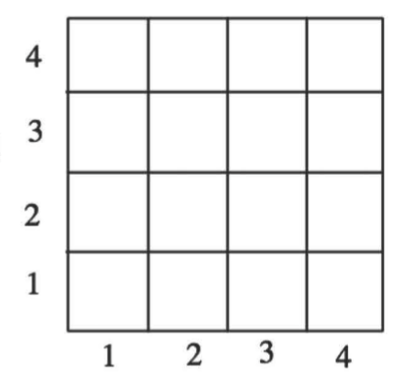
\includegraphics[width=0.45\textwidth]{L1_tworolls.png}
\eci 
}
{
\bci [$\circ$]
\item<3-> \empr {Continuous case:} Dropping a needle in a plain

\bigskip
- $\Omega = \{(x,y) \in \real^2 \mid 0 \le x,y \le 1 \}$

\bigskip
\centering
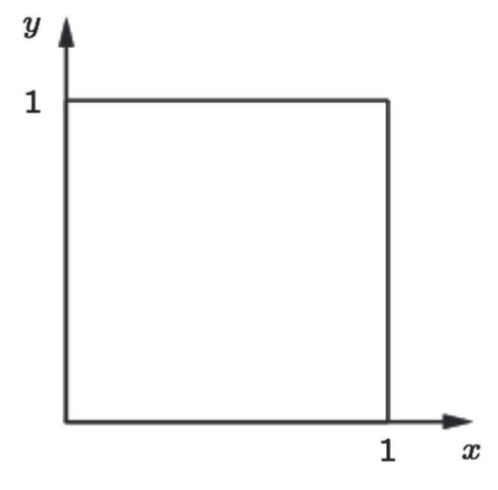
\includegraphics[width=0.5\textwidth]{L1_needle.png}
\eci 
}

\end{frame}

%%%%%%%%%%%%%%%%%%%%%%%%%%%%%%%%%%%%%%%%%%%%%%%%%%%%%%
\begin{frame}{2. Probability Law}

\plitemsep 0.1in

\bci [$\bullet$]

\item<2-> Assign numbers to what? Each outcome?

\item<3-> What is the probability of dropping a needle at $(0.5, 0.5)$ over the $1\times 1$ plane? 

\item<4-> Assign numbers to each \redblank{5}{subset} of $\Omega$

\item<6-> a subset of $\Omega$: \redblank{7}{an event}

\item<8-> $\cprob{A}$: Probability of an event $A.$

\bci
\item This is where probability meets set theory.  
\eci

\item<9-> Roll a dice. What is the probability of odd numbers?

\medskip
$
\cprob{ \{1,3,5 \}},
$
where $\{1,3,5 \} \subset \Omega$ is an event.
\eci

\end{frame}

%%%%%%%%%%%%%%%%%%%%%%%%%%%%%%%%%%%%%%%%%%%%%%%%%%%%%%
\section{L1(3)}
\begin{frame}{Roadmap}
% \tableofcontents
%\plitemsep 0.1in
\bce[(1)]
\item \grayf{Probabilistic Model}

\item \grayf{Sample Space, Event, Probability Law}

\item \redf{Probability Axioms}
\ece
\end{frame}


%%%%%%%%%%%%%%%%%%%%%%%%%%%%%%%%%%%%%%%%%%%%%%%%%%%%%%
\begin{frame}{How should we construct $\cprob{\cdot}$?}

\plitemsep 0.1in

\bci [$\bullet$]

\item Need to construct $\cprob{\cdot}$ that naturally satisfies the intention of a probability theory designer just like you. What about the followings as starting points? 

\medskip

\bci
\item<2-> $\cprob{A} \geq 0$ for any event $A \subset \Omega$

\item<3-> $\cprob{A \cup B} = \cprob{A} + \cprob{B} - \cprob{A \cap B}$

\item<3-> $\cprob{A \cup B} \leq  \cprob{A} + \cprob{B}$ 

\item<3-> For two disjoint\footnote{Their intersection is empty.} events $A$ and $B$, $\cprob{A \cup B} = \cprob{A} + \cprob{B}$

\item<4-> $\cprob{\Omega} = 1$ (Why not $\cprob{\Omega} = 10$?)

\item<4-> $\cprob{\emptyset} = 0$

\item<5-> If $A \subset B,$ $\cprob{A} \leq \cprob{B}$

\item<5-> many others
\eci
\eci

\end{frame}

%%%%%%%%%%%%%%%%%%%%%%%%%%%%%%%%%%%%%%%%%%%%%%%%%%%%%%
\begin{frame}{Probability Axioms}

\plitemsep 0.1in

\bci 

\item<1-> Surprisingly, we need just the following three rules (called \redf{axioms}):

\medskip

\onslide<2->
{
\begin{block}{Probability Axioms: Version 1}

\bce[{A}1.] 
\item \redf{Nonnegativity:} $\cprob{A} \geq 0$ for any event $A \subset \Omega$
\item \redf{Normalization:} $\cprob{\Omega} = 1$
\item \redf{(Finite) additivity:} For two disjoint events $A$ and $B$, $\cprob{A \cup B} = \cprob{A} + \cprob{B}$
\ece
\end{block}
}

\item<3-> No other things are necessary, and we can prove all other 
things from the above axioms.

\item<4-> Note that coming up with the above axioms is far from trivial. 

\eci

\end{frame}

%%%%%%%%%%%%%%%%%%%%%%%%%%%%%%%%%%%%%%%%%%%%%%%%%%%%%%
\begin{frame}{Examples}
A1: \orangef{Nonnegativity}, A2: \orangef{Normalization}, A3: \orangef{Finite additivity}

Prove the following properties using the axioms: \hfill \only<1>{\lecturemark{VIDEO PAUSE}}

\plitemsep 0.1in

%\abovedisplayskip=-0.1in

\bce 
\item For any event $A,$ $\cprob{A} \leq 1$
\aleq{
\onslide<2->{1 \overset{\text{A2}}{=} \cprob{\Omega} = \cprob{A \cup A^c}} \onslide<3->{\overset{\text{A3}}{=} \cprob{A} + \cprob{A^c}} \onslide<4->{\imp \cprob{A} = 1 - \cprob{A^c}} \onslide<5->{\overset{\text{A1}}{\le} 1}
}

\item $\cprob{\emptyset} = 0$
\aleq{
\onslide<6->{\cprob{\Omega \cup \emptyset} \overset{\text{A3}}{=} \cprob{\Omega} + \cprob{\emptyset}} \onslide<7->{\overset{\text{A2}}{=} 1+ \cprob{\emptyset}} \onslide<8->{\overset{\text{from 1.}}{\imp} \cprob{\emptyset} =0}
}

\item If $A \subset B,$ $\cprob{A} \leq \cprob{B}$
\aleq{
\onslide<9->{\cprob{B} \overset{\text{A3}}{=}} \onslide<10->{\cprob{A} + \cprob{B \setminus A} \overset{\text{A1}}{\ge} \cprob{A}}
}
\ece

\end{frame}

%%%%%%%%%%%%%%%%%%%%%%%%%%%%%%%%%%%%%%%%%%%%%%%%%%%%%%
\begin{frame}{Probability Calculation Steps}


\mytwocols{0.5}{
\mbox{}
\medskip

\plitemsep 0.1in
\bce 
\item Specify the sample space
\item Specify a probability law

- from my earlier belief, from data, from expert's opinion

\item Identify an event of interest
\item Calculate
\ece
}
{
Toss a (biased) coin

\plitemsep 0.1in

\bce
\item $\Omega = \{H,T \}$ 

\item $\cprob{\{H \}} = 1/4,$ $\cprob{\{T \}} = 3/4,$

\item probability of head or tail

\item 1/4, 3/4
\ece
}
\end{frame}

%%%%%%%%%%%%%%%%%%%%%%%%%%%%%%%%%%%%%%%%%%%%%%%%%%%%%%
\begin{frame}{Discrete but infinite sample space}


\plitemsep 0.07in

\bci
\item $\Omega = \{1,2, 3, \ldots \},$  $\cprob{\{ n \}} = \frac{1}{2^n},$ $n=1,2, \ldots$ 

\item<2-> Is the above probability law legitimate? \orangef{seems OK}
\onslide<3->
{
\aleq{
\cprob{\Omega} = \frac{1}{2} + \frac{1}{2^2} + \cdots = \frac{1/2}{1-1/2} = 1
}}
\vspace{-0.3cm}
\item<4-> $\cprob{\text{even numbers}}$?
\onslide<5->
{
\begin{align*}
 \cprob{\text{even}} 
 &= \cprob{\{2,4, 6, \ldots \}} \cr    
 &= \frac{1}{2^2} + \frac{1}{2^4} + \frac{1}{2^6} + \cdots = 1/3
\end{align*}}

\item<6-> Is the above right? If not, why?
\bci
\item<7-> Wrong: \redf{Finite} additivity axiom does not allow this.
\eci

\eci

\end{frame}

%%%%%%%%%%%%%%%%%%%%%%%%%%%%%%%%%%%%%%%%%%%%%%%%%%%%%%
\begin{frame}{Probability Axioms Version \only<1>{1} \only<2>{2}}

\begin{block}{Probability Axioms: Version \only<1>{1} \only<2>{2}}
\plitemsep 0.1in
\bce[{A}1.] 
\item Nonnegativity: $\cprob{A} \geq 0$ for any event $A \subset \Omega$
\item Normalization: $\cprob{\Omega} = 1$

\only<1>{\item \redf{(Finite) additivity:} For two disjoint events $A$ and $B$, $\cprob{A \cup B} = \cprob{A} + \cprob{B}$}

\only<2>{\item \redblk{Countable additivity:} If $A_1, A_2, A_3, \ldots$ is an infite sequence of disjoint events, then $\cprob{A_1 \cup A_2 \cup \cdots} = \cprob{A_1} + \cprob{A_2} + \cdots.$}
\ece
\end{block}

% \plitemsep 0.1in
% \bci
% \item 
% \item 
% \eci

\end{frame}

%%%%%%%%%%%%%%%%%%%%%%%%%%%%%%%%%%%%%%%%%%%%%%%%%%%%%%
\begin{frame}{Interpretation of Probability Theory}


\plitemsep 0.1in
\bci
\item<1-> A narrow view: A branch of math

\bci
\item axioms $\rightarrow$ theorems
\item Mathematicians work very hard to find the smallest set of necessary axioms (just like atoms in physics)
\eci



\item<2-> Frequencies: $\cprob{H} = 1/2$
\bci
\item Understanding an uncertain situation: fractions of successes out of many experiments

\eci


\item<3-> Beliefs: $\cprob{\text{He is reelected}} = 0.7$

\eci

\medskip
Anyway, we believe that probabilistic reasoning is very helpful to understand the world with many uncertain situations.
\end{frame}


%%%%%%%%%%%%%%%%%%%%%%%%%%%%%%%%%%%%%%%%%%%%%%%%%%%%%%
\begin{frame}{}
\vspace{2cm}
\LARGE Questions?


% \medskip
% \LARGE Congratulations! You build up the very basics of a probabilistic model. 

% \medskip

% \LARGE What else do we need to build up?
\end{frame}

%%%%%%%%%%%%%%%%%%%%%%%%%%%%%%%%%%%%%%%%%%%%%%%%%%%%%%
\begin{frame}{}
\vspace{2cm}
% \LARGE Questions?


\medskip
\LARGE You build up the very basics of a probabilistic model. 

\medskip

\LARGE What else do we need to build up?
\end{frame}

%%%%%%%%%%%%%%%%%%%%%%%%%%%%%%%%%%%%%%%%%%%%%%%%%%%%%%
\begin{frame}{Review Questions}
% \tableofcontents
%\plitemsep 0.1in
\bce[1)]
\item Please explain what a probabilistic model is and why we need it. 

\item What is the mathematical definition of event?

\item What are the key elements of the probabilistic model?

\item Please list up the probability axioms and explain them. 

\item Why do we need countable additivity in the probability axioms?

\ece
\end{frame}


\end{document}

